\documentclass[12pt,a4paper]{report}

% WildSnake CS3104 mini-project report. Replace the marked identity fields
% and add genuine screenshots before submission.
\usepackage[margin=25mm]{geometry}
\usepackage[T1]{fontenc}
\usepackage{lmodern}
\usepackage{microtype}
\usepackage{graphicx}
\usepackage{xcolor}
\usepackage{listings}
\usepackage{booktabs}
\usepackage{longtable}
\usepackage{array}
\usepackage{enumitem}
\usepackage{float}
\usepackage{hyperref}
\usepackage{tikz}
\usetikzlibrary{arrows.meta,positioning,shapes.geometric,fit,calc}

\hypersetup{colorlinks=true,linkcolor=blue!50!black,urlcolor=blue!60!black}
\setlength{\parindent}{0pt}
\setlength{\parskip}{0.55em}
\renewcommand{\arraystretch}{1.2}
\definecolor{codebg}{RGB}{247,248,250}
\definecolor{codeblue}{RGB}{30,75,135}
\lstdefinestyle{cpp}{
  language=C++, basicstyle=\ttfamily\small, keywordstyle=\color{codeblue}\bfseries,
  commentstyle=\color{gray}, stringstyle=\color{green!35!black},
  numbers=left, numberstyle=\tiny\color{gray}, numbersep=8pt,
  breaklines=true, showstringspaces=false, frame=single,
  backgroundcolor=\color{codebg}, rulecolor=\color{gray!35},
  columns=fullflexible, keepspaces=true, tabsize=4
}
\lstset{style=cpp}

\tikzset{
  uml/.style={draw,rounded corners,align=center,minimum width=28mm,
              minimum height=10mm,font=\small,fill=blue!4},
  actor/.style={draw,ellipse,align=center,minimum width=20mm,
                minimum height=9mm,font=\small,fill=orange!10},
  flow/.style={-{Stealth[length=2.2mm]},thick},
  rel/.style={-{Stealth[length=2mm]},thick},
  activity/.style={draw,rounded corners,align=center,minimum width=37mm,
               minimum height=8mm,font=\small,fill=blue!4},
  decision/.style={draw,diamond,aspect=2.0,align=center,inner sep=2pt,
                   font=\small,fill=yellow!15}
}

\begin{document}
\begin{titlepage}
  \centering
  {\Large \textbf{INDIAN INSTITUTE OF INFORMATION TECHNOLOGY TIRUCHIRAPALLI}}\\[3mm]
  {\large Department of Computer Science and Engineering}\\[18mm]
  {\Huge\bfseries WildSnake}\\[3mm]
  {\Large Snake Game Engine: Object-Oriented Design and Implementation}\\[18mm]
  {\large Mini Project Report}\\[2mm]
  {\large Course: CS3104 -- Object-Oriented Programming in C++}\\[16mm]
  \begin{tabular}{c@{\hspace{18mm}}c}
    \textbf{Student 1} & \textbf{Student 2}\\[3mm]
    \large Sampath Kumar Reddy & \large Syed Adam\\[2mm]
    Roll No. 251158 & Roll No. 251156
  \end{tabular}\\[12mm]
  \begin{tabular}{>{\bfseries}p{43mm}p{75mm}}
    Academic year and semester: & 2nd Year, Semester 3\\
    Submission date: & 29 October 2026
  \end{tabular}\\[20mm]
  \vfill
  {\large Final project report}
\end{titlepage}

\pagenumbering{roman}
\chapter*{Declaration}
We declare that the project contribution described in this report, titled
\textit{WildSnake}, was developed as a CS3104 mini project. The implementation
details and limitations are reported to the best of our knowledge. Any external
libraries used are identified in the report. The student authors are listed on
the cover page.

\vspace{15mm}
\begin{tabular}{p{70mm}p{70mm}}
  \rule{60mm}{0.4pt} & \rule{60mm}{0.4pt}\\
  Sampath Kumar Reddy & Syed Adam\\
  Roll No. 251158 & Roll No. 251156\\[3mm]
  Date: 29 October 2026 & Date: 29 October 2026
\end{tabular}

\chapter*{Acknowledgement}
We thank the course instructor for the instruction and feedback provided
during this mini project. (Edit this section to acknowledge any additional
contributors.)

\chapter*{Abstract}
WildSnake is a small snake-game engine implemented in C++17 and presented
through a browser interface. The engine models the snake, food, board, score,
and game state as separate C++ classes. A lightweight HTTP server exposes
state, direction, tick, and reset operations to a JavaScript front end. The
project demonstrates encapsulation, composition, an abstract observer
interface, standard-library containers, and separation between game rules and
presentation. The repository also contains a CMake build and a set of
assertion-style tests. The report documents the current source structure and
does not claim that the project has been compiled or that the tests have passed.

\textbf{Keywords:} C++, object-oriented programming, game engine, Snake, REST API,
UML, CMake

\tableofcontents
\listoffigures
\listoftables
\clearpage
\pagenumbering{arabic}

\chapter{Introduction}
\section{Background}
Snake is a grid-based game in which the player steers a growing snake to collect
food while avoiding the board boundary and the snake's own body. Its compact
rules make it useful for demonstrating state, object collaboration, input
validation, collision checks, and separation of responsibilities.

\section{Project overview}
WildSnake separates the rule engine from the graphical interface. The C++
backend owns the authoritative game state. An HTTP API lets the front end read
the state and request direction changes, game ticks, and resets. The interface
uses HTML, CSS, and JavaScript with a canvas for the board.

\section{Problem statement}
The project aims to provide a maintainable, small-scale implementation of the
classic Snake rules, with a clear object-oriented model and a usable interface.
The design should make core entities and their responsibilities understandable
to a student reviewing OOP concepts.

\section{Objectives}
\begin{itemize}[leftmargin=*]
  \item Model game entities with focused C++ classes and private state.
  \item Implement movement, direction validation, food placement, scoring, and
        collision/game-over behavior.
  \item Expose game operations through a small JSON HTTP API.
  \item Provide keyboard, on-screen, start, pause, and restart controls.
  \item Document the architecture and test the core behavior.
\end{itemize}

\chapter{Scope and Requirements}
\section{Scope}
The current implementation has a rectangular, non-wrapping board, a snake
starting at the board center, randomly placed food, score increments when food
is eaten, and game-over detection for wall, self, and obstacle collisions.
The world contains an obstacle collection, although the current constructor
does not populate it. The browser UI supports arrow keys and WASD, clickable
direction buttons, pause/resume, and restart. The backend listens on
\texttt{127.0.0.1:8080}.

The score manager can load and save a high score in a text file, but it is not
connected to the \texttt{Game} score lifecycle. The browser's high-score
presentation therefore should not be described as integrated persistent
scoring without further implementation and verification.

\section{Functional requirements}
\begin{table}[H]
\centering
\caption{Functional requirements reflected in the current source}
\begin{tabular}{p{18mm}p{115mm}}
\toprule
ID & Requirement\\\midrule
FR-01 & Display current game state, including board dimensions, snake, food,
        obstacles, score, and game-over flag.\\
FR-02 & Accept one of four cardinal direction requests.\\
FR-03 & Advance the snake one cell per tick and check collisions.\\
FR-04 & Increase the score and place new food when the snake reaches food.\\
FR-05 & Reset the snake and score and resume active play.\\
FR-06 & Allow browser controls by keyboard and on-screen buttons.\\
FR-07 & Support pause/resume in the front-end game loop.\\
FR-08 & Load and save a high score through the standalone ScoreManager class.\\
\bottomrule
\end{tabular}
\end{table}

\section{Non-functional requirements}
The code targets C++17 and uses CMake. The engine should keep game rules
independent from browser rendering, validate board dimensions and directions,
and provide readable class interfaces. The server uses a mutex around shared
game operations. Third-party dependencies declared by CMake are cpp-httplib and
nlohmann-json.

\section{Use cases}
\begin{figure}[H]
\centering
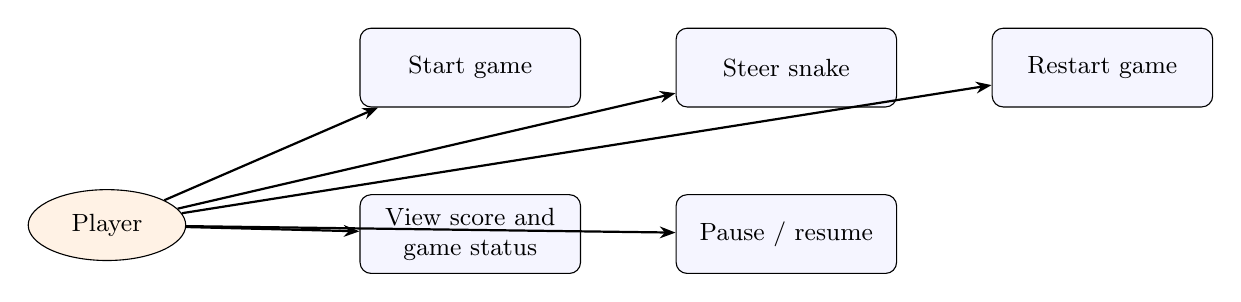
\begin{tikzpicture}[node distance=11mm and 12mm]
  \node[actor] (player) {Player};
  \node[uml,right=22mm of player,yshift=20mm] (start) {Start game};
  \node[uml,right=of start] (play) {Steer snake};
  \node[uml,below=of play] (pause) {Pause / resume};
  \node[uml,below=of start] (status) {View score and\\game status};
  \node[uml,right=of play] (restart) {Restart game};
  \draw[rel] (player) -- (start);
  \draw[rel] (player) -- (play);
  \draw[rel] (player) -- (pause);
  \draw[rel] (player) -- (status);
  \draw[rel] (player) -- (restart);
\end{tikzpicture}
\caption{Use-case view of player interactions}
\label{fig:usecase}
\end{figure}

\chapter{Design and Architecture}
\section{Layered architecture}
\begin{figure}[H]
\centering
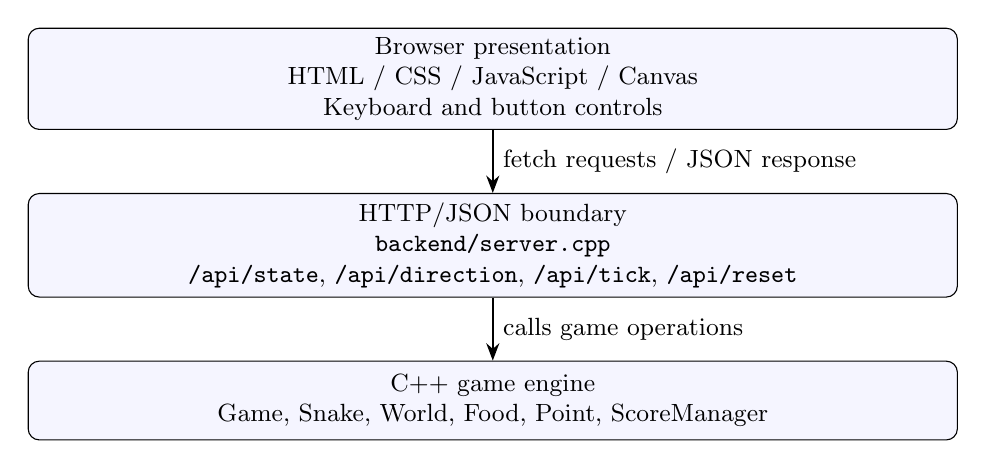
\begin{tikzpicture}[node distance=8mm]
  \node[uml,minimum width=118mm] (ui) {Browser presentation\\HTML / CSS / JavaScript / Canvas\\Keyboard and button controls};
  \node[uml,minimum width=118mm,below=of ui] (api) {HTTP/JSON boundary\\\texttt{backend/server.cpp}\\\texttt{/api/state}, \texttt{/api/direction}, \texttt{/api/tick}, \texttt{/api/reset}};
  \node[uml,minimum width=118mm,below=of api] (engine) {C++ game engine\\Game, Snake, World, Food, Point, ScoreManager};
  \draw[flow] (ui) -- node[right,font=\small]{fetch requests / JSON response} (api);
  \draw[flow] (api) -- node[right,font=\small]{calls game operations} (engine);
\end{tikzpicture}
\caption{WildSnake high-level architecture}
\label{fig:architecture}
\end{figure}

\section{Class design and OOP concepts}
\begin{itemize}[leftmargin=*]
  \item \textbf{Encapsulation:} game state is held in private members and read
        through public methods such as \texttt{getScore()} and \texttt{getBody()}.
  \item \textbf{Composition:} \texttt{Game} owns a \texttt{Snake} and a
        \texttt{World}; \texttt{World} owns a \texttt{Food} value.
  \item \textbf{Abstraction and runtime polymorphism:} \texttt{GameObserver}
        declares virtual event callbacks, and \texttt{Game} calls them through
        the interface. A concrete observer can be supplied by a client.
  \item \textbf{Standard library:} \texttt{std::deque<Point>} represents the
        body, vectors represent obstacles and occupied cells, and
        \texttt{std::mt19937} supports randomized food placement.
  \item \textbf{Value type:} \texttt{Point} represents a coordinate and defines
        equality operators used by collision and collection logic.
\end{itemize}

\begin{figure}[H]
\centering
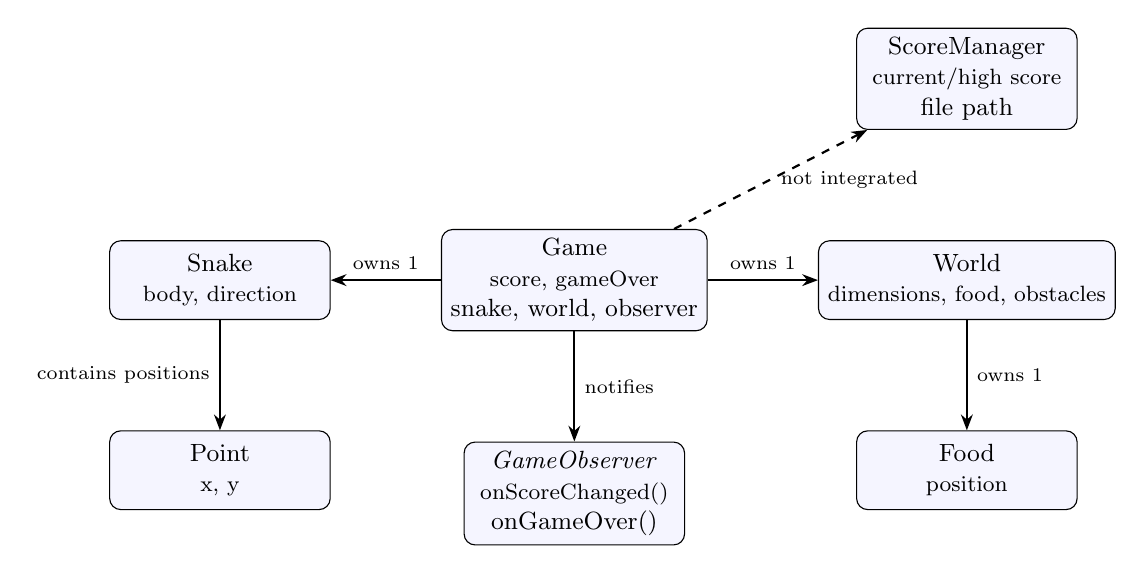
\begin{tikzpicture}[node distance=14mm and 14mm]
  \node[uml] (game) {Game\\\footnotesize score, gameOver\\snake, world, observer};
  \node[uml,left=of game] (snake) {Snake\\\footnotesize body, direction};
  \node[uml,right=of game] (world) {World\\\footnotesize dimensions, food, obstacles};
  \node[uml,below=of world] (food) {Food\\\footnotesize position};
  \node[uml,below=of snake] (point) {Point\\\footnotesize x, y};
  \node[uml,below=of game] (obs) {\textit{GameObserver}\\\footnotesize onScoreChanged()\\onGameOver()};
  \node[uml,above=of world] (score) {ScoreManager\\\footnotesize current/high score\\file path};
  \draw[rel] (game) -- node[above,font=\scriptsize]{owns 1} (snake);
  \draw[rel] (game) -- node[above,font=\scriptsize]{owns 1} (world);
  \draw[rel] (world) -- node[right,font=\scriptsize]{owns 1} (food);
  \draw[rel] (snake) -- node[left,font=\scriptsize]{contains positions} (point);
  \draw[rel] (game) -- node[right,font=\scriptsize]{notifies} (obs);
  \draw[rel,dashed] (game) -- node[right,font=\scriptsize]{not integrated} (score);
\end{tikzpicture}
\caption{Core class relationships. ScoreManager is currently standalone.}
\label{fig:class}
\end{figure}

\section{UML class specification tables}
The following UML-style tables list the declared attributes and public
operations for every class in the game model. A minus sign denotes private
visibility and a plus sign denotes public visibility. The \texttt{GameObserver}
callbacks are virtual; \texttt{ScoreManager} remains a separate utility in the
current implementation.

\small
\begin{longtable}{p{28mm}p{54mm}p{73mm}}
\caption{UML class table: model data types and entities}\label{tab:uml-entities}\\
\toprule
Class & Attributes (visibility) & Public operations (visibility)\\
\midrule
\endfirsthead
\toprule Class & Attributes (visibility) & Public operations (visibility)\\
\midrule
\endhead
\bottomrule
\endfoot
\texttt{Point} & \texttt{x: int}, \texttt{y: int} (public value fields) &
\texttt{Point(x=0,y=0)}; \texttt{operator==}; \texttt{operator!=}.\\
\texttt{Direction} (enum) & Values: \texttt{UP}, \texttt{DOWN},
\texttt{LEFT}, \texttt{RIGHT} & Scoped enumeration used by \texttt{Snake}
and the API.\\
\texttt{Snake} & \texttt{body\_: deque<Point>}, \texttt{direction\_: Direction},
\texttt{growing\_: bool} (private) & \texttt{Snake(start)};
\texttt{getBody()}; \texttt{getDirection()}; \texttt{setDirection()};
\texttt{move()}; \texttt{grow()}; \texttt{occupies()}; \texttt{hitsItself()}.\\
\texttt{Food} & \texttt{position\_: Point} (private) & \texttt{Food(position)};
\texttt{getPosition()}; \texttt{setPosition()}.\\
\texttt{Grid<T>} & \texttt{width\_: int}, \texttt{height\_: int},
\texttt{cells\_: vector<T>} (private) & \texttt{Grid(width,height)};
\texttt{getWidth()}; \texttt{getHeight()}; \texttt{contains(Point)};
\texttt{at(Point)} (mutable and const overloads). Methods are declared in the
header; definitions are absent from the supplied source.\\
\texttt{World} & \texttt{width\_: int}, \texttt{height\_: int},
\texttt{food\_: Food}, \texttt{obstacles\_: vector<Point>},
\texttt{rng\_: mt19937} (private) & \texttt{World(width,height)};
\texttt{getWidth()}; \texttt{getHeight()}; \texttt{getFood()};
\texttt{getObstacles()}; \texttt{isInside(Point)}; \texttt{hasObstacle(Point)};
\texttt{placeFood(occupied)}.\\
\end{longtable}
\normalsize

\small
\begin{longtable}{p{28mm}p{54mm}p{73mm}}
\caption{UML class table: game coordination and score utility}\label{tab:uml-services}\\
\toprule
Class & Attributes (visibility) & Public operations (visibility)\\
\midrule
\endfirsthead
\toprule Class & Attributes (visibility) & Public operations (visibility)\\
\midrule
\endhead
\bottomrule
\endfoot
\texttt{GameObserver} (abstract interface) & No data members declared &
\texttt{onScoreChanged(score)} (public pure virtual);
\texttt{onGameOver()} (public pure virtual); virtual destructor.\\
\texttt{Game} & \texttt{snake\_: Snake}, \texttt{world\_: World},
\texttt{score\_: int}, \texttt{gameOver\_: bool},
\texttt{observer\_: unique\_ptr<GameObserver>} (private) &
\texttt{Game(width,height)}; \texttt{setObserver()}; \texttt{changeDirection()};
\texttt{tick()}; \texttt{reset()}; \texttt{getScore()}; \texttt{isGameOver()};
\texttt{getSnake()}; \texttt{getWorld()}.\\
\texttt{ScoreManager} & \texttt{currentScore\_: int}, \texttt{highScore\_: int},
\texttt{filePath\_: string} (private) & \texttt{ScoreManager(filePath)};
\texttt{resetCurrentScore()}; \texttt{addPoints(points)};
\texttt{getCurrentScore()}; \texttt{getHighScore()}; \texttt{loadHighScore()};
\texttt{saveHighScore() const}. This utility is not currently composed into
\texttt{Game}.\\
\end{longtable}
\normalsize

\section{Sequence: one game tick}
\begin{figure}[H]
\centering
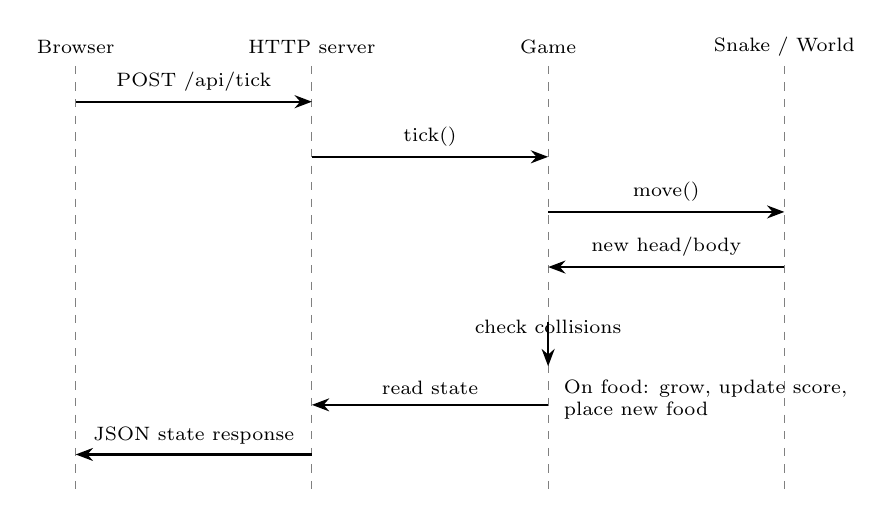
\begin{tikzpicture}[x=1cm,y=0.7cm, every node/.style={font=\scriptsize}]
  \node (browser) at (0,0) {Browser};
  \node (server) at (3,0) {HTTP server};
  \node (game) at (6,0) {Game};
  \node (snake) at (9,0) {Snake / World};
  \foreach \x in {0,3,6,9} \draw[dashed,gray] (\x,-0.35) -- (\x,-8.1);
  \draw[flow] (0,-1) -- node[above]{POST /api/tick} (3,-1);
  \draw[flow] (3,-2) -- node[above]{tick()} (6,-2);
  \draw[flow] (6,-3) -- node[above]{move()} (9,-3);
  \draw[flow] (9,-4) -- node[above]{new head/body} (6,-4);
  \draw[flow] (6,-5) -- node[above]{check collisions} (6,-5.8);
  \draw[flow] (6,-6.5) -- node[above]{read state} (3,-6.5);
  \draw[flow] (3,-7.4) -- node[above]{JSON state response} (0,-7.4);
  \node[align=left] at (8,-6.4) {On food: grow, update score,\\place new food};
\end{tikzpicture}
\caption{Sequence for a browser-requested game tick}
\label{fig:sequence}
\end{figure}

\section{Activity: tick and collision handling}
\begin{figure}[H]
\centering
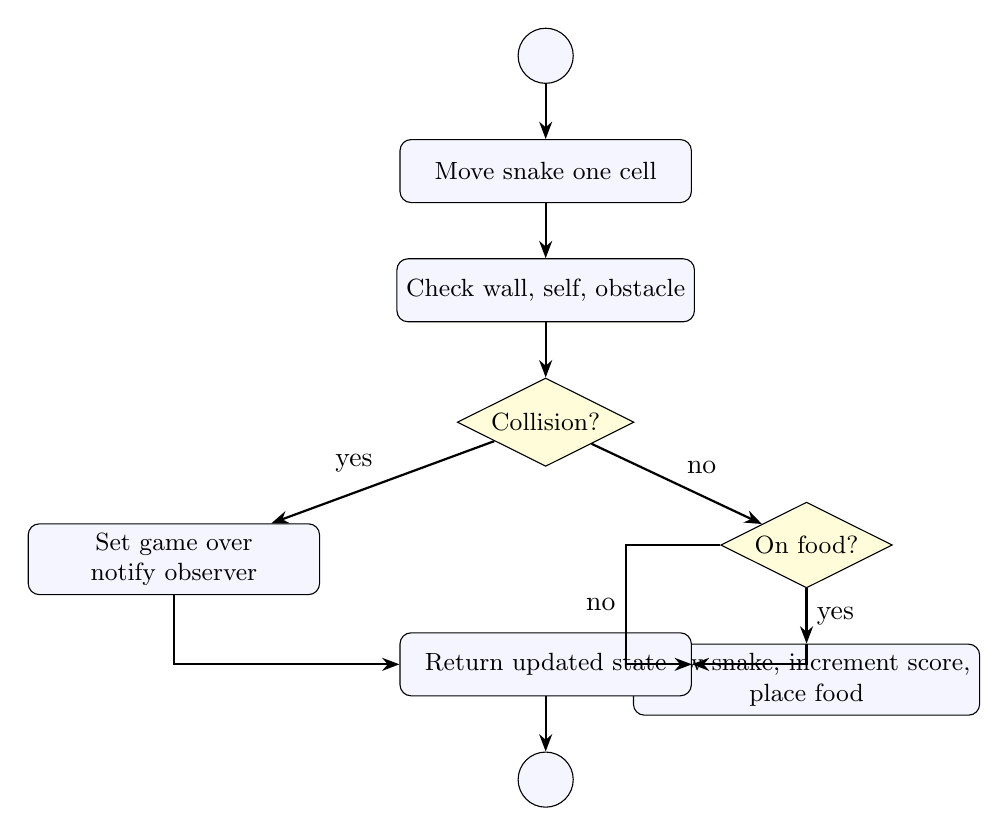
\begin{tikzpicture}[node distance=7mm]
  \node[uml,circle,minimum size=7mm,inner sep=0pt] (begin) {};
  \node[activity,below=of begin] (move) {Move snake one cell};
  \node[activity,below=of move] (collision) {Check wall, self, obstacle};
  \node[decision,below=of collision] (dead) {Collision?};
  \node[activity,below left=10mm and 23mm of dead] (over) {Set game over\\notify observer};
  \node[decision,below right=10mm and 22mm of dead] (food) {On food?};
  \node[activity,below=of food] (score) {Grow snake, increment score,\\place food};
  \node[activity,below=21mm of dead] (done) {Return updated state};
  \node[uml,circle,below=of done,minimum size=7mm,inner sep=0pt] (end) {};
  \draw[flow] (begin) -- (move);
  \draw[flow] (move) -- (collision);
  \draw[flow] (collision) -- (dead);
  \draw[flow] (dead) -- node[above left]{yes} (over);
  \draw[flow] (dead) -- node[above right]{no} (food);
  \draw[flow] (over) |- (done);
  \draw[flow] (food) -- node[right]{yes} (score);
  \draw[flow] (food.west) -- ++(-12mm,0) |- node[left,pos=0.25]{no} (done.east);
  \draw[flow] (score) |- (done);
  \draw[flow] (done) -- (end);
\end{tikzpicture}
\caption{Activity diagram for a game tick}
\label{fig:activity}
\end{figure}

\chapter{Implementation}
\section{Technology stack}
WildSnake uses a lightweight browser frontend and a C++17 backend. The
frontend is implemented with native browser technologies and does not use a
JavaScript framework. The C++ game engine owns the authoritative gameplay
state; an HTTP/JSON interface carries input requests to the engine and returns
state for the browser to render.

\begin{table}[H]
\centering
\caption{Technology stack and its role in WildSnake}
\label{tab:technology-stack}
\begin{tabular}{p{39mm}p{96mm}}
\toprule
Technology & Role in the project\\\midrule
C++17 and standard library & Implement the game engine and model. The project
uses containers such as \texttt{deque} and \texttt{vector}, random-number
utilities, smart pointers, file streams, and a mutex.\\
HTML5 and CSS3 & Structure and style the browser interface.\\
JavaScript and Canvas & Handle keyboard and button input, call the backend,
run the browser game loop, and draw the board and game entities.\\
HTTP and JSON & Connect the frontend and backend through the state, direction,
tick, and reset endpoints.\\
cpp-httplib & Provide the lightweight C++ HTTP server; CMake fetches version
0.18.3.\\
 nlohmann-json & Parse and serialize JSON in the server; CMake fetches version
3.12.0.\\
CMake and CTest & Configure the C++17 build and register the game test
executable. The presence of the test target does not by itself confirm that
the tests pass.\\
Python 3 & Serve the static frontend locally during development using Python's
HTTP server.\\
Browser local storage & Store the high-score value shown by the frontend;
this is separate from the standalone C++ \texttt{ScoreManager}.\\
Git and GitHub & Track source changes and host the project repository.\\
\bottomrule
\end{tabular}
\end{table}

The backend dependencies are declared in \texttt{backend/CMakeLists.txt} and
are fetched by CMake. The project uses no frontend framework: the browser
modules are plain JavaScript files that communicate with the local C++ server
at \texttt{127.0.0.1:8080}.

\subsection{Project modules}
\begin{table}[H]
\centering
\caption{Project modules}
\begin{tabular}{p{35mm}p{96mm}}
\toprule
Module & Responsibility\\\midrule
\texttt{Snake} & Body, direction validation, movement, growth, self-collision.\\
\texttt{World} and \texttt{Food} & Bounds, obstacles, food position, randomized placement.\\
\texttt{Game} & Coordinates ticks, collisions, score, reset, observer notifications.\\
\texttt{ScoreManager} & Reads/writes persistent high score in a text file.\\
\texttt{server.cpp} & Serializes state as JSON and routes HTTP operations.\\
Frontend & Canvas rendering, controls, API calls, and game-loop presentation.\\
Tests & Small executable covering points, snake, world, grid, and basic game state.\\
\bottomrule
\end{tabular}
\end{table}

\section{Representative OOP code}
The following excerpts are drawn from the current source with formatting
normalized for the report.

\subsection{Encapsulated game model and observer abstraction}
\begin{lstlisting}[caption={Game owns collaborators and exposes a narrow interface},label={lst:gameclass}]
class GameObserver {
public:
    virtual void onScoreChanged(int score) = 0;
    virtual void onGameOver() = 0;
    virtual ~GameObserver() = default;
};

class Game {
private:
    Snake snake_;
    World world_;
    int score_;
    bool gameOver_;
    std::unique_ptr<GameObserver> observer_;
public:
    void tick();
    void reset();
    int getScore() const;
    bool isGameOver() const;
};
\end{lstlisting}

\subsection{Direction validation and movement}
\begin{lstlisting}[caption={Snake validates directions and moves its deque body},label={lst:snake}]
void Snake::setDirection(Direction direction)
{
    switch (direction) {
        case Direction::UP: case Direction::DOWN:
        case Direction::LEFT: case Direction::RIGHT:
            break;
        default:
            throw std::invalid_argument("Invalid snake direction");
    }
    // A multi-segment snake cannot reverse into itself.
    if (body_.size() > 1 && isOpposite(direction_, direction))
        return;
    direction_ = direction;
}

void Snake::move()
{
    Point head = body_.front();
    advance(head, direction_);
    body_.push_front(head);
    if (growing_) growing_ = false;
    else body_.pop_back();
}
\end{lstlisting}
\textit{Note:} \texttt{isOpposite} and \texttt{advance} above are explanatory
helpers; the repository implements these checks directly in the method body.

\subsection{Tick orchestration and composition}
\begin{lstlisting}[caption={Game coordinates movement, collisions, and food handling},label={lst:tick}]
void Game::tick()
{
    if (gameOver_) return;
    snake_.move();
    checkCollisions();
    if (gameOver_) return;

    if (snake_.getBody().front() == world_.getFood().getPosition()) {
        snake_.grow();
        updateScore();
        // Build occupied cells and request the next food position.
        world_.placeFood(occupiedCells());
    }
}
\end{lstlisting}
\textit{Note:} \texttt{occupiedCells()} abbreviates the vector construction in
the source; the repository builds that vector from the snake body.

\section{HTTP API}
\begin{table}[H]
\centering
\caption{Backend API operations}
\begin{tabular}{p{27mm}p{34mm}p{72mm}}
\toprule
Method & Path & Behavior\\\midrule
GET & \texttt{/api/state} & Returns dimensions, snake, food, obstacles, score, gameOver.\\
POST & \texttt{/api/direction} & Accepts JSON \texttt{\{"direction":"UP"\}}; rejects invalid input.\\
POST & \texttt{/api/tick} & Advances one step and returns updated state.\\
POST & \texttt{/api/reset} & Resets the engine and returns new state.\\
GET & \texttt{/} & Returns server name/status and endpoint names.\\
\bottomrule
\end{tabular}
\end{table}

\chapter{Testing and Results}
\section{Test approach}
The repository contains \texttt{tests/game\_tests.cpp}, a standalone test
program registered with CTest when \texttt{BUILD\_TESTING} is enabled. Its
checks cover point equality, initial and changed snake movement, invalid
direction rejection, world boundaries and minimum size, grid access, initial
game state, one tick, and reset. The test file expresses checks by printing
PASS/FAIL and returning a failing exit code if any check fails.

\section{Test status and observed repository limitations}
The report was prepared by source inspection; no build or test execution is
claimed. Before submission, compile the project and record the actual command,
environment, and result here. At source inspection, there are case/name
inconsistencies that may prevent a clean build on case-sensitive systems:
\texttt{point.h} versus includes of \texttt{Point.h}, and
\texttt{ScoreMananger.h} versus includes of \texttt{ScoreManager.h}. Also,
\texttt{Grid<T>} declares template methods in \texttt{World.h}, but their
definitions are not present in the supplied source files even though the tests
instantiate \texttt{Grid<int>}. Resolve these and rerun the tests before
submitting.

\begin{table}[H]
\centering
\caption{Coverage in the existing test source (not a claim of passing tests)}
\begin{tabular}{p{54mm}p{70mm}}
\toprule
Area & Checks represented\\\midrule
Point & Equality and inequality.\\
Snake & Initial position, movement, direction change, self-hit baseline,
invalid direction.\\
World and Grid & In-bounds checks, minimum dimensions, element access and
out-of-range behavior.\\
Game & Initial score/state, one tick, score/state after reset.\\
Additional recommended cases & Eat/grow/score, wall collision, self-collision,
reverse-direction prevention, no free food cells, observer callbacks, server
request validation.\\
\bottomrule
\end{tabular}
\end{table}

\section{Screenshots}
\begin{figure}[H]
\centering
\IfFileExists{report-assets/game-start.png}{
  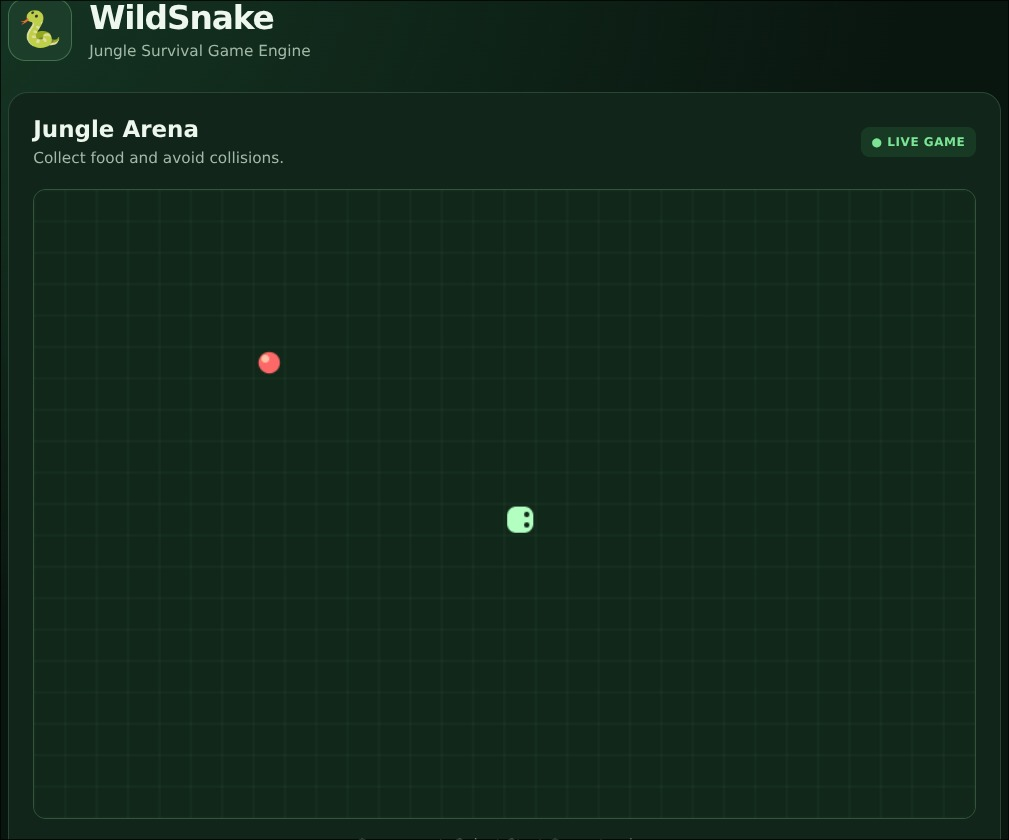
\includegraphics[width=0.88\textwidth]{report-assets/game-start.png}
}{\fbox{\parbox[c][45mm][c]{0.82\textwidth}{\centering
  Insert screenshot: running WildSnake at initial state\\
  Save as \texttt{report-assets/game-start.png}}}}
\caption{WildSnake initial game screen}
\label{fig:screenshot-start}
\end{figure}

\begin{figure}[H]
\centering
\IfFileExists{report-assets/game-over.png}{
  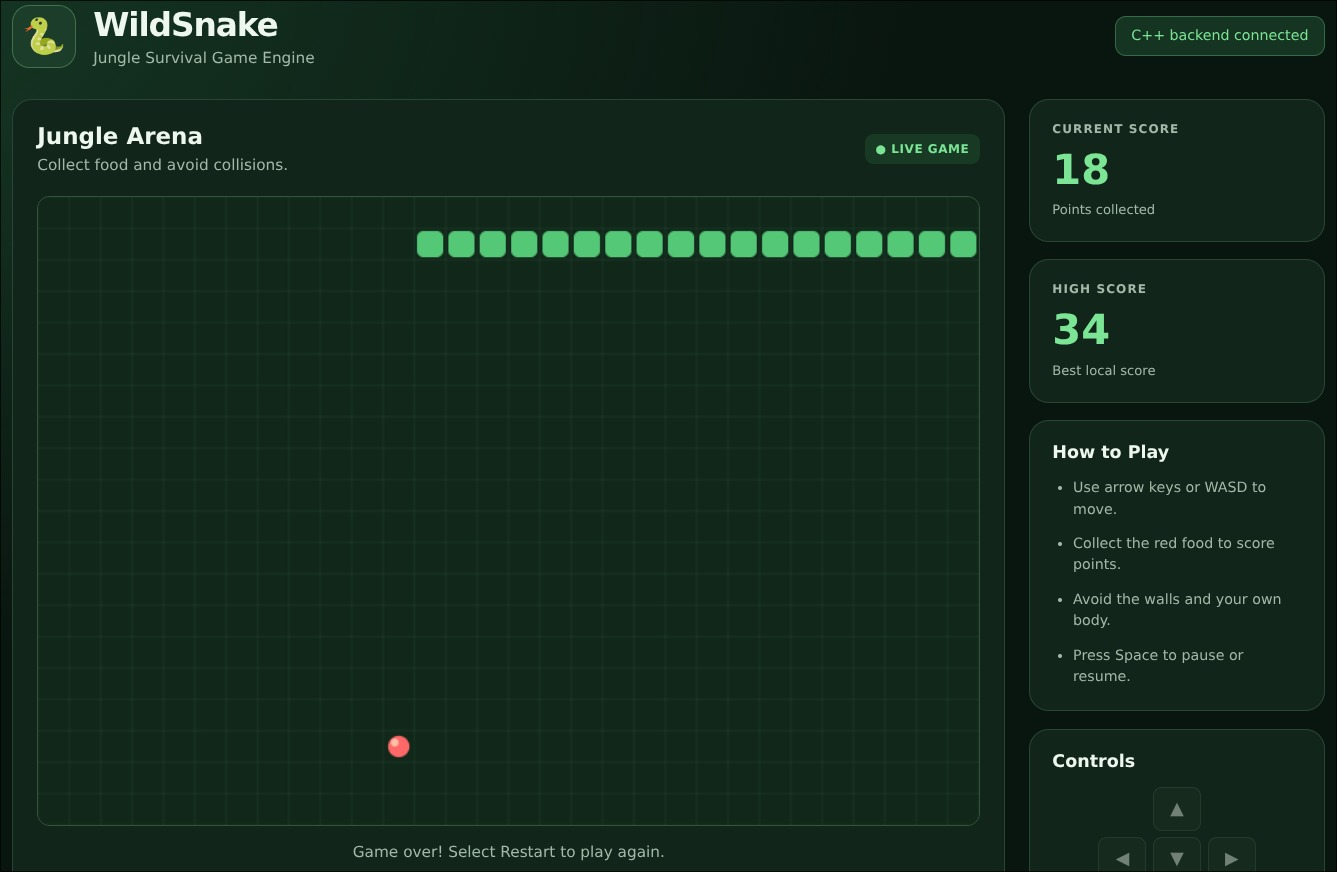
\includegraphics[width=0.88\textwidth]{report-assets/game-over.png}
}{\fbox{\parbox[c][45mm][c]{0.82\textwidth}{\centering
  Insert the supplied game-over screenshot here\\
  Save as \texttt{report-assets/game-over.png}}}}
\caption{WildSnake game-over screen showing a score of 18 and a high score of 34}
\label{fig:screenshot-game-over}
\end{figure}

\chapter{Conclusion and Future Work}
WildSnake is a useful OOP mini-project foundation: its engine is divided into
small classes, exposes a browser API, and represents core gameplay concepts
with private state and explicit interfaces. The TikZ diagrams describe the
intended relationships and the current tick flow. The test source covers
several basic cases, but the build and test outcome still needs to be verified.

Recommended next steps are to fix include/file-name consistency, implement or
remove the currently undefined Grid template, connect persistent score
management if high-score behavior is a requirement, and add tests for food,
growth, collisions, and observer notifications. Further extensions could add
configurable obstacles, difficulty levels, sound, and a packaged release.

\chapter*{References}
\addcontentsline{toc}{chapter}{References}
\begin{enumerate}[leftmargin=*]
  \item ISO C++ Foundation, ``C++ documentation,'' \url{https://isocpp.org/}.
  \item CMake, ``CMake Documentation,'' \url{https://cmake.org/documentation/}.
  \item yhirose, ``cpp-httplib,'' \url{https://github.com/yhirose/cpp-httplib}.
  \item nlohmann, ``JSON for Modern C++,'' \url{https://github.com/nlohmann/json}.
  \item TikZ and PGF, ``TikZ and PGF Manual,'' \url{https://tikz.dev/}.
  \item WildSnake project source code, supplied project repository, accessed
        [enter date].
\end{enumerate}

\appendix
\chapter{Build and Run Guide}
The CMake configuration declares the C++17 engine, HTTP server, smoke
executable, and CTest target. From the project root, a typical build sequence
is shown below. Dependency fetching may require network access at configure
time. Run these commands after correcting the source naming and Grid issues;
record the actual results in Chapter 6.
\begin{lstlisting}[language=bash,basicstyle=\ttfamily\small]
cmake -S backend -B build -DBUILD_TESTING=ON
cmake --build build
ctest --test-dir build --output-on-failure
\end{lstlisting}

\chapter{Submission Completion Checklist}
\begin{itemize}[leftmargin=*]
  \item Replace the institution name and repository access date if required by
        the department's format.
  \item Add genuine application screenshots in \texttt{report-assets/}.
  \item Fix the noted source/build issues and run the build and tests; report
        actual outcomes.
  \item Confirm the instructor's supplied template and apply any required
        cover-page, certificate, or formatting changes. The template mentioned
        in the request was not present in the workspace or chat attachment.
  \item Compile this file with a LaTeX installation that includes TikZ and
        listings, and inspect the generated PDF for layout and diagram issues.
\end{itemize}

\end{document}
